\begin{figure}
\begin{leftfullpage}
\caption[Functional connectivities for PV--/--, PV--/+, and PV+/+ cell pairs]
{{\bf Functional connectivities for PV--/--, PV--/+, and PV+/+ cell pairs}

Top panels (A,C, and E) show aspects of functional connectivity expressed through conventional noise correlations. 
Bottom panels (B, D, and F) show connectivity expressed through regularized partial noise correlations.
Data points represent averages for each of $n=11$ sites conditioned on cell pair type.
Overall, partial noise correlations provide stronger effects and greater discriminability of cell pair types.

{\bf A.} Average noise correlations. 

{\bf B.} Average partial noise correlations.   

{\bf C.} Rates of positive (green) and (negative) connectivity obtained by thresholding the correlations to make a sparse matrix of interactions.  
The sparsities was matched to matrices in panel D.

{\bf D.} Rates of positive (green) and (negative) connectivity in the sparse component of the partial correlation estimates.

{\bf E.} The ratios of positive connectivity rates to negative connectivity rates based on  thresholded correlations.

{\bf F.} The ratios of positive  connectivity rates to negative connectivity rates based on the sparse component of partial correlation estimates.

}\label{fig:pv2}
\end{leftfullpage}
\end{figure}

\begin{figure}
\begin{fullpage}
\begin{center}
    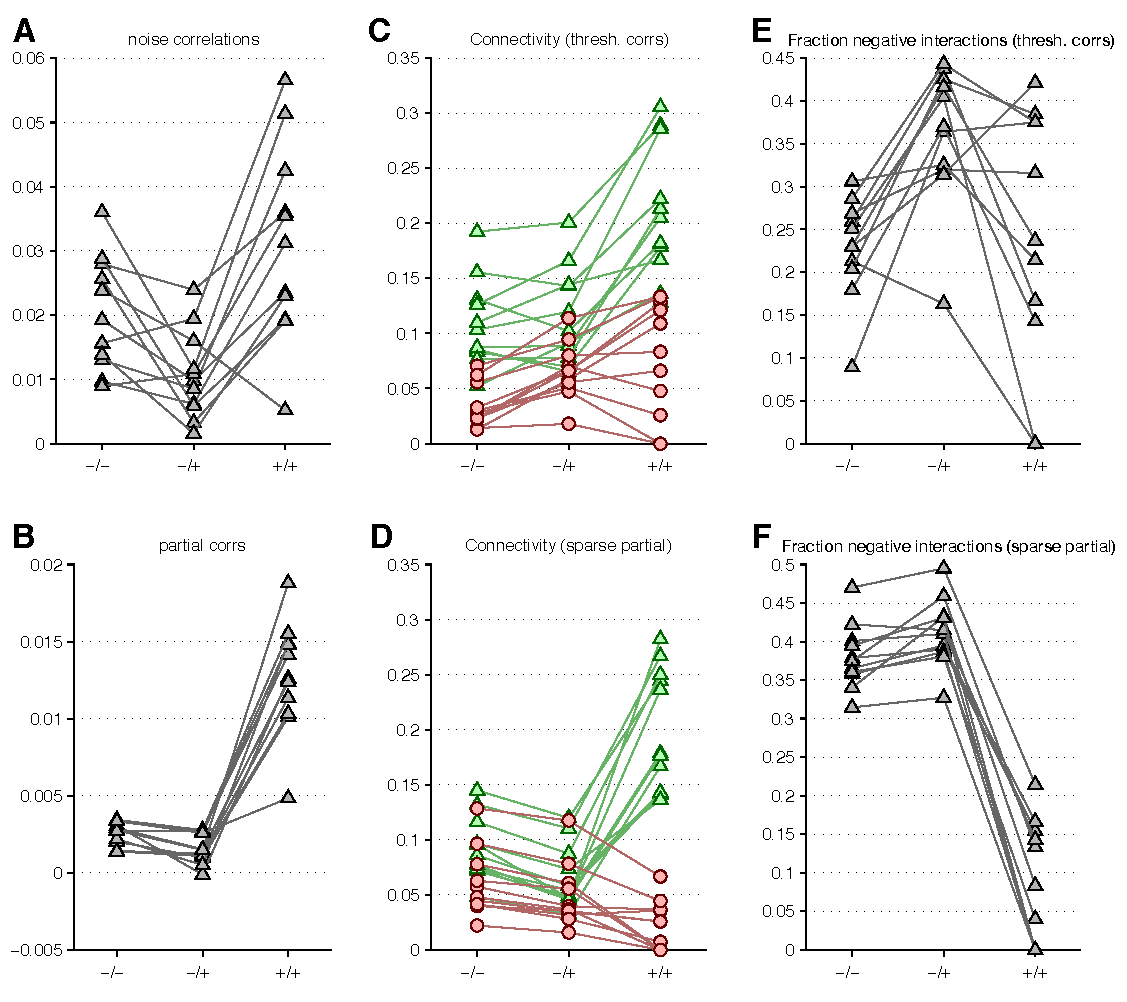
\includegraphics[width=\textwidth]{./figures/pv-fig2.pdf}
\end{center}
\end{fullpage}
\end{figure}
